% Chapter Template

\chapter{Introduction} % Main chapter title
\label{Chapter1} % for referencing this chapter elsewhere, use \cref{Chapter1}
In the recent past decades, the cancer incidence has steadily increased, affecting more than X millions of people. As shown in Figure \ref{fig:asryears}A, the incidence rate has been ever on the rise. Nonetheless, the curve of the mortality rate is dropping since the early 1990s, suggesting more effective treatments have been developed and improved over the last 20 years. Nowadays, several methods are employed to heal this disease: surgery, radiotherapy, chemotherapy, hormone therapy, targeted therapy, immunotherapy and cell-based approaches, and nuclear medicine. To achieve an effective removal of this disease, a combination of these techniques is typically applied to treat the patient. However, 

Figure XB shows both the incidence and mortality rates per 100 000 cases with respect to the body organ affected. 

Tailored treatments is currently the next step to advance further in curing cancer. The cancer relapse still represent the major cause of death. 

\begin{figure}[h!]
	\centering
	
\includegraphics[width=1.0\linewidth]{../Figures/ASR_years}
	\caption{Cancer age-standardized rate (ASR) of European Countries since the beginning of the second half of the 20th century. Data retrieved from GLOBOCAN 2022 (ref).}
	\label{fig:asryears}
\end{figure}


\begin{figure}[h!]
	\raggedright
	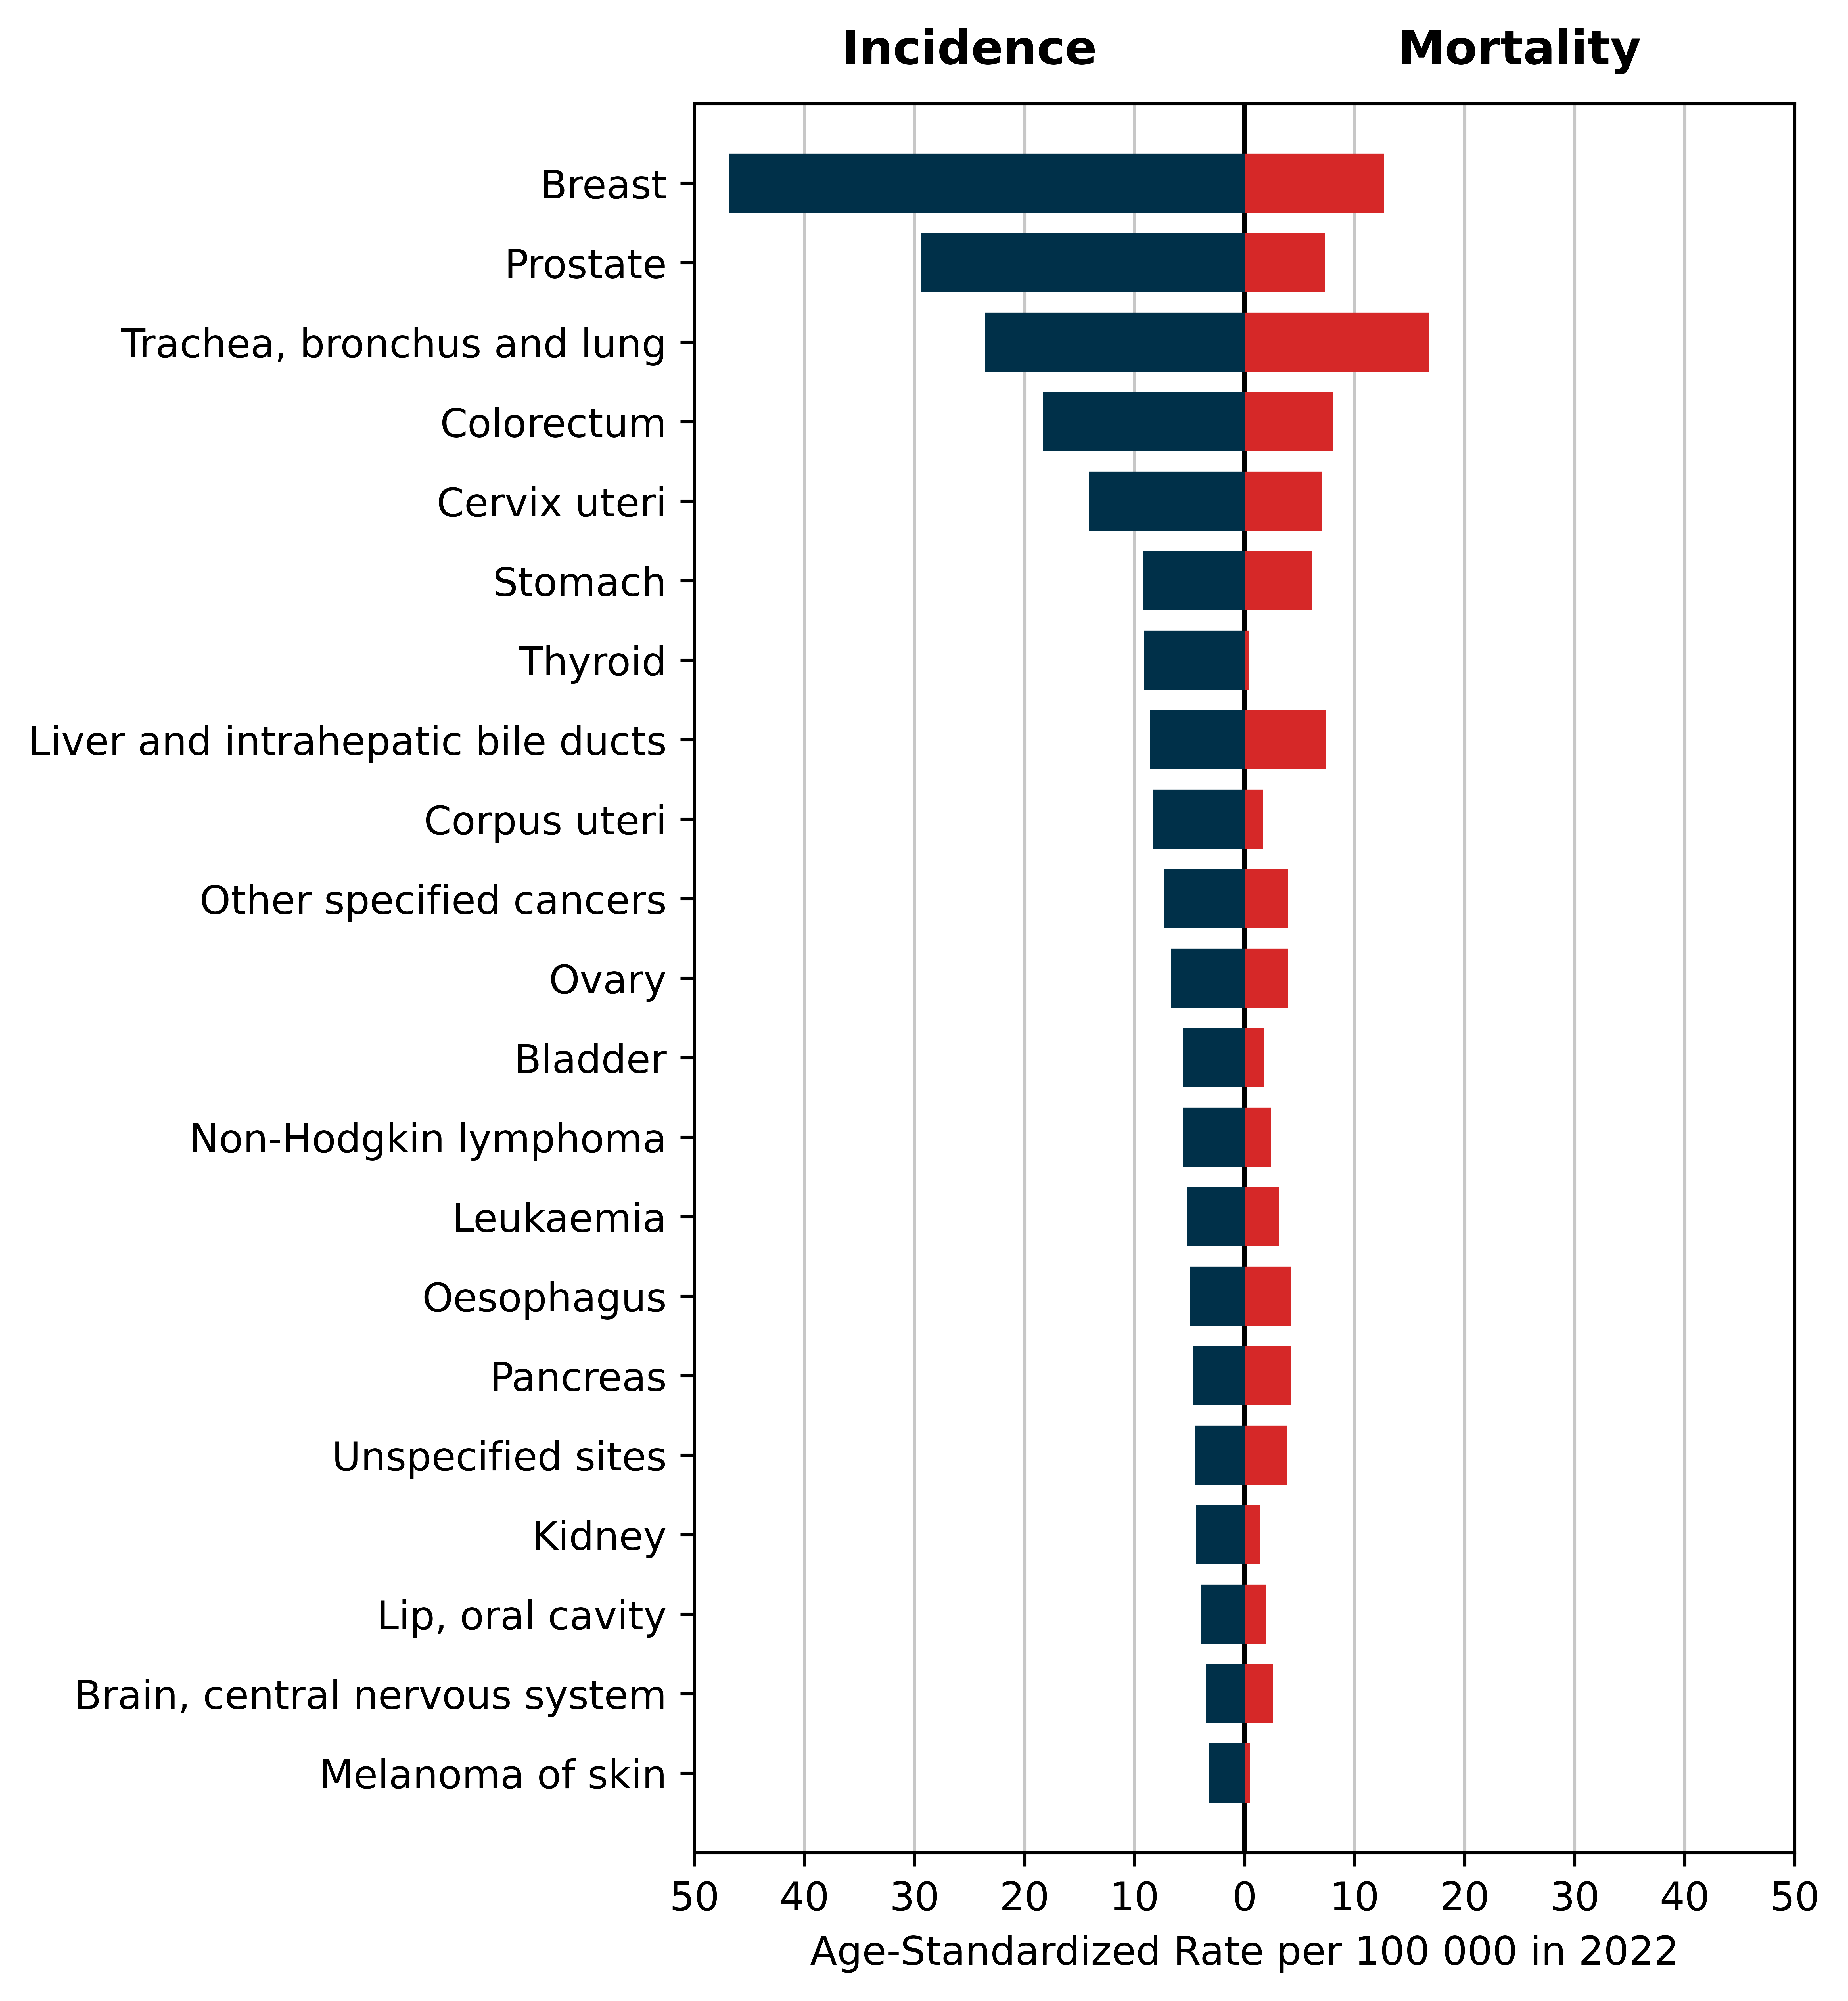
\includegraphics[width=0.7\linewidth]{../Figures/ASR_cancer}
	\caption{Incidence and mortality cancer age-standardized rate (ASR) worldwide grouped according to the organs affected. Data retrieved from GLOBOCAN 2022 (ref).}
	\label{fig:asrcancer}
\end{figure}


\section{Nuclear Medicine}
Intro nuclear medicine

\subsection{Diagnosis}

\subsection{Therapy}
